\documentclass[12pt,a4paper]{article}

% for polish language
\usepackage{polski}

% for some math symbols
\usepackage{amssymb}

% correct footnotes placement
\usepackage[bottom]{footmisc}

% for \say command
\usepackage{dirtytalk}

% change title of the bibliography
\def\bibname{Referencje}\let\refname\bibname

% for advanced math formulas
\usepackage{mathtools}
% define ceil and floor
\DeclarePairedDelimiter\ceil{\lceil}{\rceil}
\DeclarePairedDelimiter\floor{\lfloor}{\rfloor}

\usepackage{listings}
% colors for snippet background
\usepackage{xcolor}

% links
\usepackage{hyperref}
% \hypersetup{
%     colorlinks,
%     citecolor=black,
%     filecolor=black,
%     linkcolor=black,
%     urlcolor=blue
% }

% image displaying
\usepackage{subcaption}
\usepackage{graphicx}

\usepackage{multirow} 
\usepackage{makecell}

% display structure of the project
\usepackage{dirtree}

% include pdf images
\usepackage{pdfpages}

% bold math
\usepackage{bm}

\title{Dokumentacja do projektu z AMHE}

\author{Roman Moskalenko \and Pavel Tarashkevich}
\date{}

\begin{document}

\maketitle
\tableofcontents
\newpage

\section{Treść zadania}

\textbf{Zadanie 10.}\\

Zaprojektuj algorytm ewolucyjny i zbadaj jego działanie w jednym z zadań zdefiniowanych w ramach środowiska OpenAI poświęconym kontroli.

Specyfikacja zadań znajduje się pod poniższym linkiem:

\href{https://gym.openai.com/envs/#classic\_control}{gym.openai.com/envs/\#classic\_control}

Porównaj wyniki swojego rozwiązania z dwoma wybranymi rozwiązaniami, które bazują na
innych podejściach.


\section{Projekt wstępny}

\subsection{Opis problemu i jego sposób rozwiązania}

Zadania kontroli klasycznej zakładają sterowanie obiektu fizycznego w sposób,
jak najbardziej efektywny dla jego stanu. Funkcja sterowania może być bardzo
skomplikowana, uciążliwe jest jej zaprojektowanie w sposób ręczny.

Algorytmy uczenia się ze wzmocnieniem (dalej RL) są wykorzystywane w zadaniach związanych z kontrolą.
Do ewaluacji tych algorytmów powstał zestaw środowisk OpenAI gym.

Alternatywnym podejściem do zadań kontroli jest bezpośrednie stosowanie sieci
neuronowych, m.i. podejście neuroewolucji zastosowane w \cite{scalable_alternative},
które zakłada połączenie sieci neuronowych i algorytmów ewolucyjnych.

Do rozwiązania tego problemu planujemy zastosować sieć MLP, gdzie wejściem sieci
będzie stan rozważanego środowiska, a wyjściem będzie akcja do wyboru przez agenta.
Sieć ta będzie optymalizowana za pomocą algorytmu ewolucyjnego CMA-ES.

\subsection{Planowane eksperymenty numeryczne}\label{subsection:planned}

W ramach eksperymentów ocenimy działanie implementacji naszego algorytmu
neuroewolucji na różnych środowiskach OpenAI gym.

Następnie porównamy jego działanie z dwoma algorytmami RL pod kątem
końcowej nagrody oraz czasu uczenia algorytmu. Wybrane przez nas
algorytmy RL to A2C oraz PPO.


\subsection{Biblioteki wybrane do realizacji projektu}\label{subsection:libs}

\begin{itemize}
  \item \textbf{\href{https://github.com/openai/gym}{gym}} - liczne środowiska, w tym kontroli klasycznej,
        do trenowania agentów.
  \item \textbf{\href{https://github.com/CyberAgentAILab/cmaes}{cmaes}} -
        implementacja algorytmu CMA-ES.
  \item \textbf{\href{https://github.com/DLR-RM/stable-baselines3}{stable-baselines}} -
        biblioteka zawierająca gotowe implementację algorytmów RL.
\end{itemize}

\pagebreak
\section{Project końcowy}

\subsection{Uzupełnienie projektu wstępnego}

Na dodatek do bibliotek wymienionych w \ref{subsection:libs} użyliśmy
biblioteki \textbf{\href{https://pytorch.org/}{PyTorch}} do implementacji
perceptronu wielowarstwowego.

\subsection{Przeprowadzone eksperymenty}

Dany rozdział opisuje szczegóły przeprowadzonych w ramach projektu
eksperymentów: opis środowisk na których działają agenty, ich uczenie i
przetestowanie.

\subsubsection{Opis środowisk kontroli klasycznej}

Do przetestowania algorytmów rozważanych w ramach projektu wykorzystane
zostały środowiska OpenAI gym \cite{openai_gym}, w szczególności dotyczące
kontroli klasycznej: środowiska powszechnie znane, proste ze względu
na działanie i rozwiązywalność.

W tabeli \ref{table:env_properties} znajdują się rozważane przez nas
środowiska oraz ich właściwości.


% 500 iterations
\begin{table}[!h]
  \begin{tabular}{lrrrr}
    \hline
    \multicolumn{1}{c}{Środowisko} & \multicolumn{1}{c}{\# obs.} & \multicolumn{1}{c}{\# akcje} & \multicolumn{1}{c}{typ akcji} & \multicolumn{1}{c}{rozwiązany dla} \\
    \hline
    CartPole-v0                    & 4                           & 2                            & dyskretna                     & 195                                \\
    CartPole-v1                    & 4                           & 2                            & dyskretna                     & 475                                \\
    MountainCar-v0                 & 2                           & 3                            & dyskretna                     & -110                               \\
    MountainCarContinuous-v0       & 2                           & 1                            & ciągła                        & 90                                 \\
    Pendulum-v1                    & 3                           & 1                            & ciągła                        & -140                               \\
    Acrobot-v1                     & 6                           & 3                            & dyskretna                     & -60                                \\
    \hline
  \end{tabular}
  \caption{
    Właściwości środowisk kontroli klasycznej. Kolumny "obs." oraz "akcje"
    wskazują wymiary zbiorów obserwacji oraz akcji odpowiednio w każdym środowisku.
    Kolumna "rozwiązanie" zawiera wartości, które wskazują granice
    nagród dla każdego środowiska, powyżej których można uznać, że agent
    zachowuje się sensownie \cite{analyzing_reinforcement} \cite{openai_gym}.
  }\label{table:env_properties}
\end{table}

\subsubsection{Metryki do porównania algorytmów}

Zgodnie z rozdziałem \ref{subsection:planned} porównujemy
algorytm neuroewolucji - połączenie CMA-ES z siecią MLP z dwoma algorytmami
RL - A2C oraz PPO.

Zdajemy sobie sprawę, że nie możemy wprost porównywać tych algorytmów, gdyż
charakter uczenia w nich jest różny: algorytm neuroewolucji uczy się
przeszukując przestrzeń parametrów sieci MLP, jedyną informacją zwrotną jest
końcowa suma nagród otrzymana na danym środowisku. Natomiast algorytmy
RL optymalizują swoją politykę zachowania na środowisku, potrafią
uwzględniać natychmiastowe nagrody, a także stany i akcje, które do nich
prowadzą.

Do porównania algorytmów uwzględniliśmy jak szybko algorytmy osiągają
kolejne sumy nagród, ile czasu zajęło uczenie. Najważniejszą metryką
porównania jest uśredniona suma nagród uzyskiwana  przez modele nauczone.

\subsubsection{Opis modeli do nauczenia}

\textbf{Algorytm neuroewolucji}: użyliśmy perceptronu
dwuwarstwowego z 8 neuronami w warstwie ukrytej. Perceptron ten nie zawiera
dodatkowych parametrów bias. Podliczyliśmy, że liczba parametrów perceptronu
będzie wystarczająco mała aby móc efektywnie stosować algorytm CMAES.
Wybraliśmy ReLU jako funkcję aktywacji.  Algorytm \mbox{CMA-ES} automatycznie
dobiera liczność populacji zgodnie ze wzorem:

\begin{equation*}
  population\_size = 4 + \floor{3 * \ln{(n)} }
\end{equation*}

gdzie $n$ to wymiar przestrzeni parametrów sieci. Przykładowo
dla $ n = 100 $ liczność populacji wynosi 17. Parametr $\sigma$
został wybrany arbitralnie i \mbox{wynosi $1.3$}.

\bigskip

\noindent\textbf{Algorytmy A2C i PPO}: użyliśmy domyślnych konfiguracji
modeli tych algorytmów z pakietu stable\_baselines3 z polityką
\emph{MlpPolicy}.

\subsubsection{Uczenie agentów}

Uczenie agentów dokonywano w ciągu 500 tysięcy kroków,
gdzie za krok uznajemy pojedynczą akcją dokonaną przez
agenta na danym środowisku.

Warto zaznaczyć, że ze względu na to, że agent
algorytmu CMAESNN korzysta z populacji osobników niezależnie
działających na środowisku, postanowiliśmy zliczać wykonane kroki tylko
przez jednego osobnika, który uzyskał największą sumę nagród
w danym epizodzie.

Uczenie jest dokonane łącznie 5 razy dla każdej pary środowisko-algorytm,
aby zmniejszyć wpływ losowości na uzyskane wyniki.

Na rysunku \ref{fig:training} pokazano jeden z pięciu przebiegów uczenia
algorytmów. Wartości na osi pionowej odpowiadają sumom nagród,
które algorytmy uzyskują na końcu epizodu działania na danym środowisku.

\begin{figure}[!h]
  \centering
  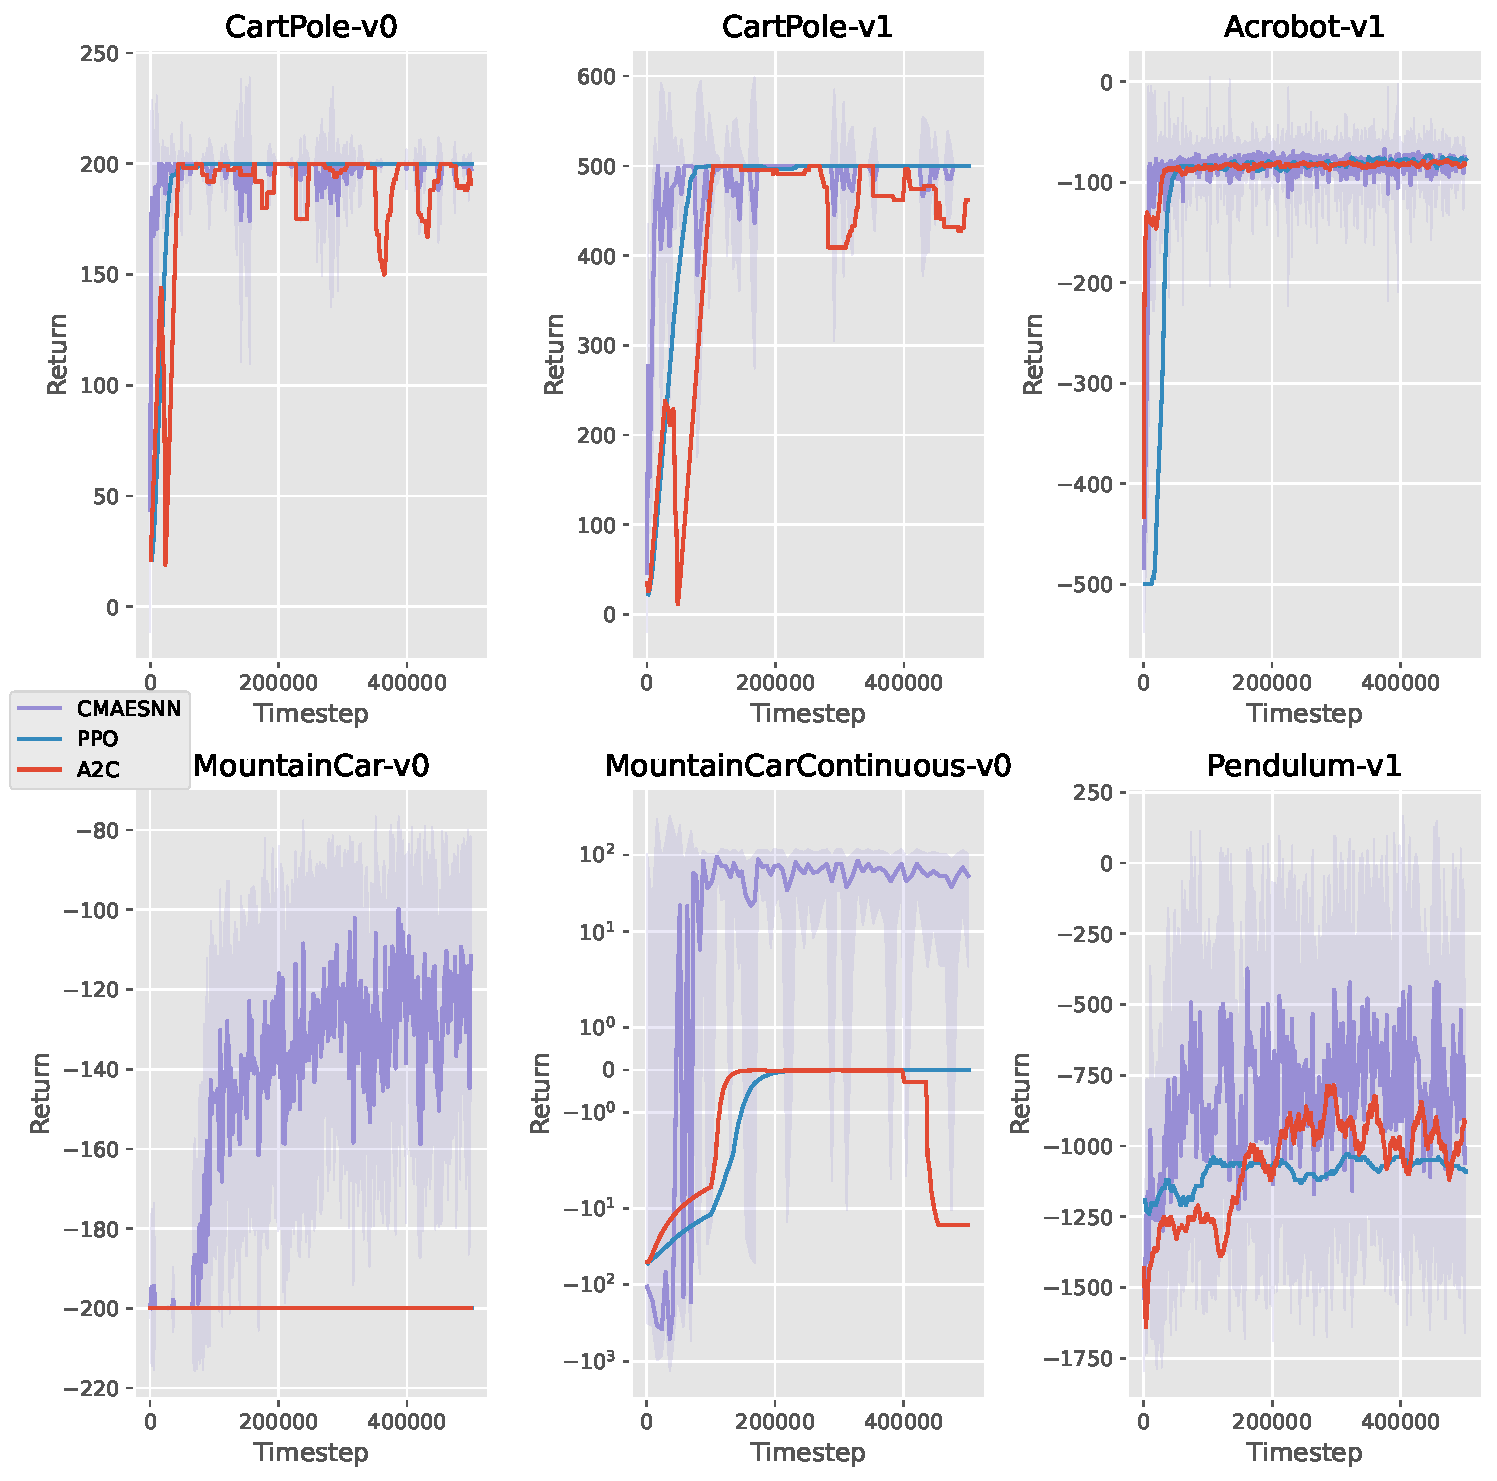
\includegraphics[width=0.7\textwidth]{../plotting/plots/plot_all0.pdf}
  \caption{Przebieg uczenia algorytmów w przeciągu 500,000 kroków.
    Dla algorytmu CMAESNN pokazano zakres sum nagród, uzyskany przez
    średnią sumę nagród oraz odchylenia standardowego dla całej populacji.}
  \label{fig:training}
\end{figure}

Jako że algorytm CMAESNN jest algorytmem przeszukiwania postanowiliśmy w trakcie
uczenia śledzić najlepszą dotychczas populację poprzez najlepszą uśrednioną wartość
sum nagród otrzymanych przez jej osobników. Dla porównania także zapisujemy
najlepsze sumę nagród dla algorytmów RL. Wartości te są podane w tabeli
\ref{table:training}.

\begin{table}[!h]
  \centering
  \hskip-1.0cm\begin{tabular}{llll}
    \hline
    \multicolumn{1}{c}{}     & \multicolumn{1}{c}{A2C}      & \multicolumn{1}{c}{PPO} & \multicolumn{1}{c}{CMAESNN}              \\
    \hline
    CartPole-v0              & \phantom{$-$}200             & \phantom{$-$}200        & \phantom{\bm{$-$}}\bm{$200$}             \\
    CartPole-v1              & \phantom{$-$}500             & \phantom{$-$}500        & \phantom{\bm{$-$}}\bm{$500$}             \\
    MountainCar-v0           & $-200$                       & $-200$                  & \bm{$-104.54 \pm 8.41$}                  \\
    MountainCarContinuous-v0 & \phantom{$-$}$0.77 \pm 1.55$ & \phantom{$-$}0.0        & \phantom{\bm{$-$}}\bm{$81.20 \pm 35.97$} \\
    Pendulum-v1              & $-843.2 \pm 237.08$          & $-1060 \pm 29.66$       & \bm{$-221 \pm 89.43$}                    \\
    Acrobot-v1               & $-80.44 \pm 2.90$            & $-73.98 \pm 1.21$       & \bm{$-67.56 \pm 0.81$}                   \\
    \hline
  \end{tabular}
  \caption{ Największę sumę nagród otrzymywane przez agentów w trakcie uczenia, uśrednione
    po pięciu przebiegach uczenia, oraz uśrednione odchylenia standardowe. Odchylenia standardowe dla CMAESNN
    nie uwzględniają odchylenia narzucanego przez rozrzut wyników w populacji.
  }\label{table:training}
\end{table}

W pierwszych trzech środowiskach - CartPole-v0, CartPole-v1, Acrobot-v1 -
wszystkie algorytmy relatywnie szybko osiągają sumy nagród, które
odpowiadają rozwiązaniu środowiska (albo bliskości do niego). Kolejne trzy -
MountainCar-v0, MountainCarContinuous-v0, Pendulum-v1 - wyraźnie sprawiają
kłopoty dla algorytmów RL. Algorytm CMAESNN dzięki wbudowanej właściwości do
eksploracji potrafi rozwiązać pierwsze dwa z nich oraz wykazuje się
lepszymi wynikami w trzecim środowisku. Warto też zwrócić uwagę na dużo
większą wariancję sum nagród w populacji dla tych środowisk.

Resztę wykresów uczenia agentów można znaleźć w dodatku
\ref{appendix:training}.

Zostały zmierzone czasy uczenia agentów. Podajemy tylko jeden wykres,
ponieważ pozostałe pomiary czasu były prawie identyczne. Na rysunku \ref{fig:training_time}
wyraźnie widać liniową zależność czasu uczenia od liczby kroków. Na większości
wykresach algorytm CMAESNN spędza dużo więcej czasu na uczenie, co
można wytłumaczyć tym, że algorytm w przeciągu epizodu przechodzi środowisko
tyle razy, ile osobników występuje w populacji. Z innej strony dana cecha
algorytmu umożliwia łatwą jego skalowalność, co jest dobrze opisane
w \cite{scalable_alternative}.

\begin{figure}[!h]
  \centering
  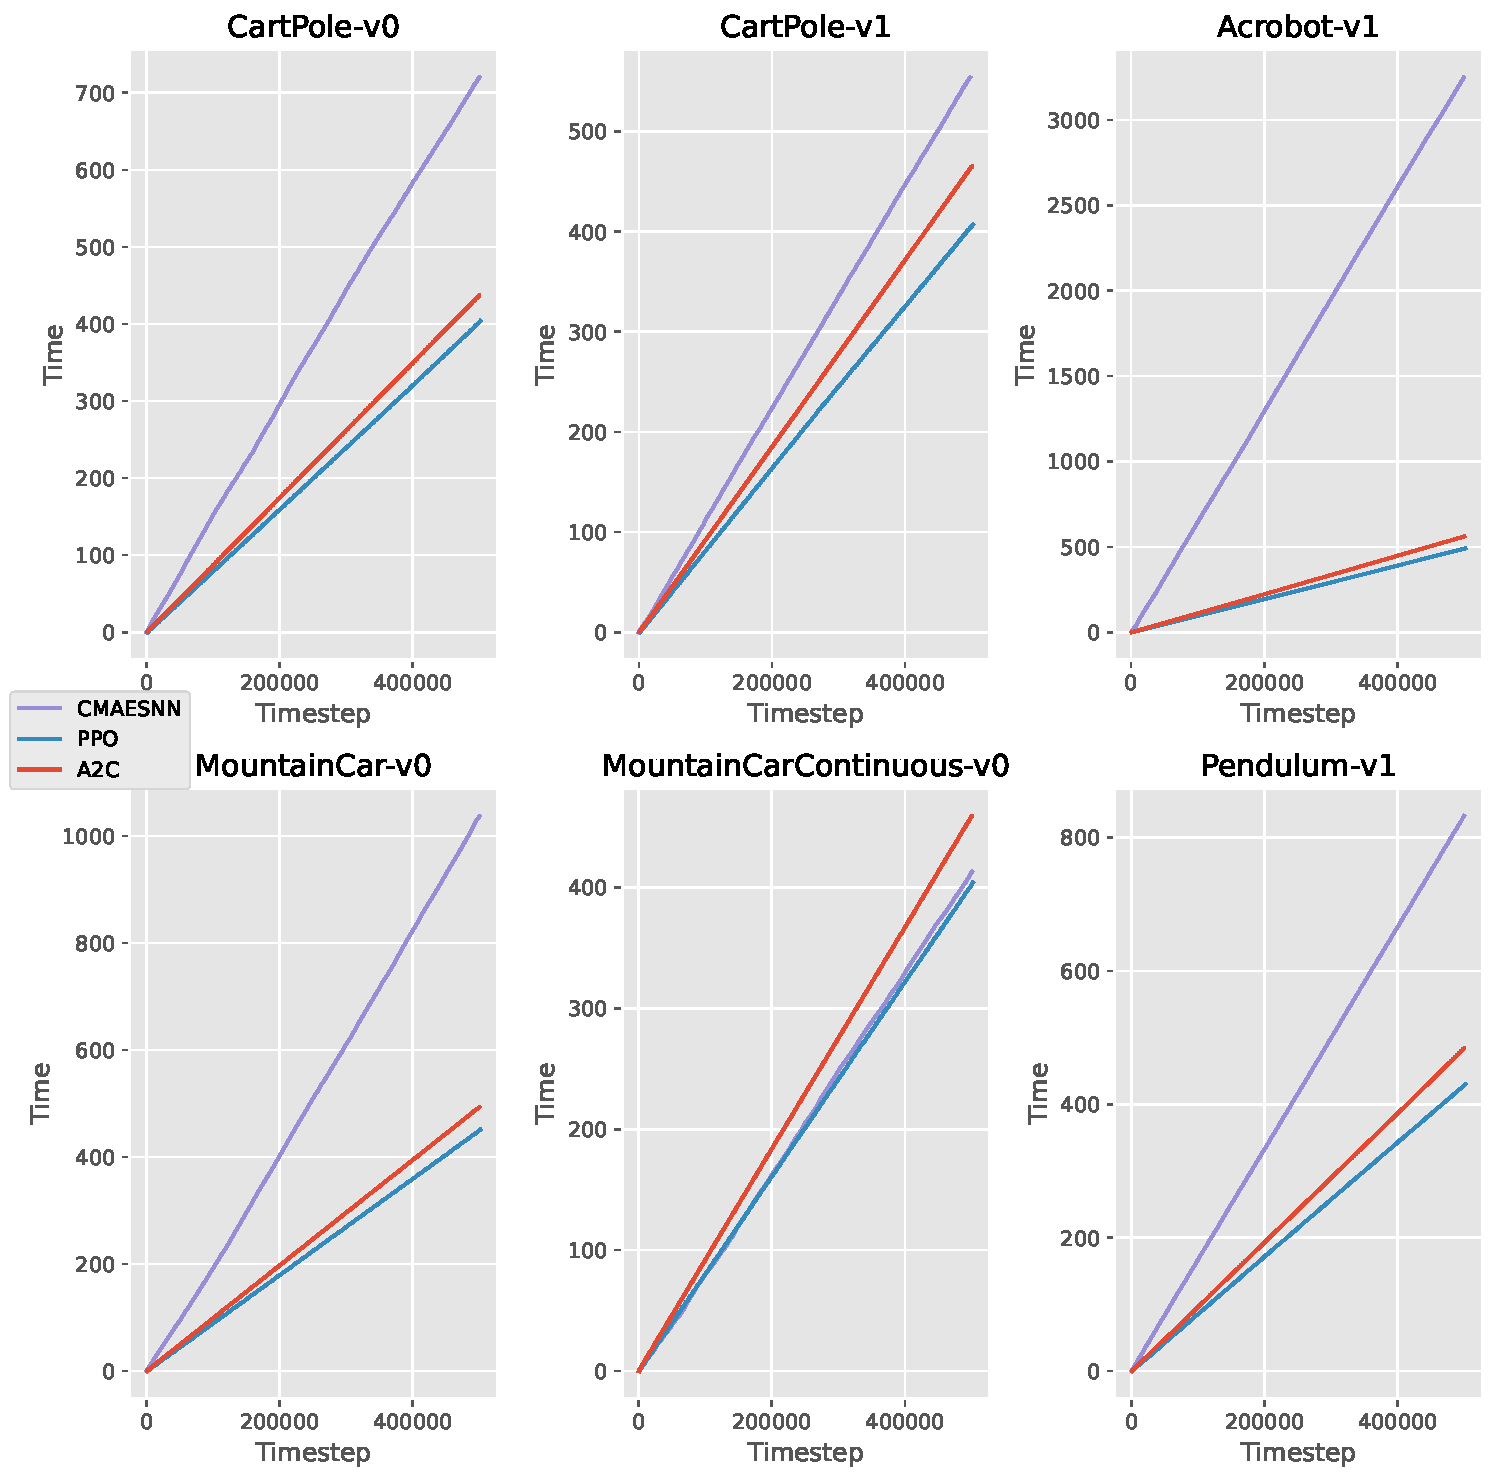
\includegraphics[width=0.7\textwidth]{../plotting/plots/plot_time0.pdf}
  \caption{Czasy uczenia ($s$) agentów w przeciągu 500,000 kroków.}
  \label{fig:training_time}
\end{figure}

\pagebreak
Ciekawostka: obecność wartości bias w implementacji sieci neuronowej
algorytmu CMAESNN negatywnie wpłynęła na działanie na środowiskach
MountainCar-v0 oraz MountainCarContinuous-v0. W dodatku \ref{appendix:bias}
można znaleźć przebiegi uczenia CMAESNN z tymi parametrami i bez nich.
Na dane zjawisko zwrócono też uwagę w \cite{analyzing_reinforcement}.

\subsubsection{Sprawność nauczonych agentów}

Po nauczeniu agentów przetestowaliśmy sprawność ich działania.
Wszystkie 5 nauczonych wersji agentów z poprzedniego rozdziału zostały
uruchomione. Uśrednione (po 10 uruchomieniach) wyniki znajdują się w tabeli
\ref{table:testing}.

\begin{table}[!h]
  \centering
  \begin{tabular}{llllr}
    \hline
    \multicolumn{1}{c}{}     & \multicolumn{1}{c}{A2C}         & \multicolumn{1}{c}{PPO} & \multicolumn{1}{c}{CMAESNN}              & \multicolumn{1}{c}{} \\
    \hline
    CartPole-v0              & \phantom{$-$}$181.28 \pm 40.90$ & \phantom{$-$}\bm{$200}$ & \phantom{\bm{$-$}}$199.7 \pm 2.1$        &                      \\
    CartPole-v1              & \phantom{$-$}$500$              & \phantom{$-$}$500$      & \phantom{\bm{$-$}}\bm{$500$}             &                      \\
    MountainCar-v0           & $-200$                          & $-200$                  & \bm{$-125.82 \pm 33.43} $                &                      \\
    MountainCarContinuous-v0 & $-0.01 \pm 0.02$                & \phantom{$-$}$0.0$      & \phantom{\bm{$-$}}\bm{$49.57 \pm 49.74$} &                      \\
    Pendulum-v1              & $-841.44 \pm 579.90$            & $-1180.94 \pm 143.50$   & \bm{$-508.85 \pm 602.58$}                &                      \\
    Acrobot-v1               & $-248 \pm 206.03$               & \bm{$-73.54 \pm 10.02$} & $-82.6 \pm 21.53$                        &                      \\
    \hline
  \end{tabular}
  \caption{ Sumy nagród nauczonych agentów uśrednione po 10 uruchomieniach
    wraz z uśrednionym odchyleniem standardowym.
  }\label{table:testing}
\end{table}

Algorytm CMAESNN sprawuje się lepiej niż algorytmy A2C i PPO w domyślnych
konfiguracjach, a co więcej rozwiązuje bądź jest bliski rozwiązania dla
wszystkich środowisk kontroli klasycznej.

\pagebreak
\subsection{Opis struktury projektu}

Kod źródłowy projektu jest umieszczony w repozytorium GitHub na stronie
\href{https://github.com/skalermo/AMHE-cmaes-classic-control}
{https://github.com/skalermo/AMHE-cmaes-classic-control}
\medskip

Na rysunku \ref{fig:dirtree} pokazana jest struktura projektu.

\begin{figure}[!ht]
  \dirtree{%
    .1 ..
    .2 .gitignore.
    .2 docs.
    .3 amhe\_docs.tex.
    .2 example.py.
    .2 models.
    .2 plotting.
    .3 log\_reader.py.
    .3 plot\_all.py.
    .3 plot\_bias\_perf.py.
    .3 plot\_time.py.
    .3 plots.
    .3 utils.py.
    .2 requirements.txt.
    .2 src.
    .3 cmaes\_nn.py.
    .3 env\_info.py.
    .3 log\_utils.py.
    .3 nn.py.
    .3 train\_all.py.
    .2 test.
    .3 \_\_init\_\_.py.
    .3 test\_cmaes\_nn.py.
    .3 test\_data.
    .4 example\_log\_a2c.txt.
    .4 example\_log\_cmaesnn.txt.
    .3 test\_log\_extraction.py.
    .3 test\_log\_utils.py.
    .3 test\_nn.py.
  }
  \caption{Struktura plików projektu}
  \label{fig:dirtree}
\end{figure}

Plik \textbf{example.py} zawiera przykładowy kod, który uruchamia nauczony
model algorytmu CMAESNN oraz wyświetla jego działanie na wybranym środowisku.
W katalogu \textbf{models} znajduje zestaw nauczonych modeli, z których
korzysta ten skrypt.\\

Kod źródłowy projektu, z którego jest zbudowany \textbf{main.py} znajduje się
w katalogu \textbf{src}:
\begin{itemize}
  \item \textbf{cmaes\_nn.py} - zawiera implementację algorytmu do rozwiązywania
        problemów kontroli klasycznej, jego interfejs jest zbliżony
        do algorytmów RL z pakietu \textbf{stable-baselines3}
        (tzn. posiada implementacje funkcji \emph{learn()}, \emph{predict()},
        \emph{load()}, \emph{save()}). \\
        Łączy w sobie stosowanie algorytmu CMA-ES oraz perceptronu wielowarstwowego.

  \item \textbf{env\_info.py} - zawiera listę nazw środowisk do problemów kontroli
        klasycznej oraz informacje o tym, czy typ akcji jest ciągły bądź dyskretny.

  \item \textbf{log\_utils.py} - zawiera funkcje pomocnicze do przetwarzania
        logów programu.

  \item \textbf{nn.py} - zawiera funkcje do zbudowania perceptronu
        wielowarstwowego, a także funkcje do przypisania wektora parametrów
        do wag perceptronu.
  \item \textbf{train\_all.py} - skrypt, który wykonuje uczenie modeli
        oraz zapisanie wyników uczenia: logów oraz wytrenowanych modeli do
        katalogów \textbf{.data/logs} oraz \textbf{.data/models} odpowiednio.
\end{itemize}

Wraz z implementacją projektu powstawały testy do sprawdzenia poprawności
jego działania. Znajdują się w katalogu \textbf{test}. \\

Katalog \textbf{plotting} zawiera skrypty do generowania wykresów na
podstawie przetworzonych logów, a także katalog z wykresami wykorzystanymi
w dokumentacji.

Katalog \textbf{docs} przechowuje dokumentację projektu.
Plik \textbf{requirements.txt} zawiera listę wymaganych do zainstalowania
bibliotek.

\subsection{Uruchomienie projektu}

Dla uruchomienia projektu niezbędne jest posiadania interpretera Python wersji co najmniej 3.8
oraz zainstalowanie bibliotek znajdujących w pliku \textbf{requirements.txt}:

\begin{lstlisting}[
  backgroundcolor = \color{lightgray},
  language=bash,
]
  $ pip install -r requirements.txt
\end{lstlisting}

\bigskip

Następnie można przykładowy skrypt za pomocą polecenia:

\begin{lstlisting}[
  backgroundcolor = \color{lightgray},
  language=bash,
]
  $ python example.py
\end{lstlisting}

Testy można uruchomić poleceniem:

\begin{lstlisting}[
  backgroundcolor = \color{lightgray},
  language=bash,
]
  $ python -m unittest discover test
\end{lstlisting}

Odpalić główny skrypt uczenia można za pomocą:

\begin{lstlisting}[
  backgroundcolor = \color{lightgray},
  language=bash,
]
  $ python src/train_all.py
\end{lstlisting}

\pagebreak
\begin{thebibliography}{9}
  \bibitem{scalable_alternative}
  Tim Salimans, Jonathan Ho, Xi Chen, Szymon Sidor, Ilya Sutskever,\\
  Evolution Strategies as a Scalable Alternative to Reinforcement Learning,
  2017, \href{https://arxiv.org/pdf/1703.03864v1.pdf}{https://arxiv.org/pdf/1703.03864v1.pdf}

  \bibitem{analyzing_reinforcement}
  Declan Oller, Tobias Glasmachers, Giuseppe Cuccu, \\
  Analyzing Reinforcement Learning Benchmarks with Random Weight Guessing,
  2020, \href{https://arxiv.org/pdf/2004.07707.pdf}{https://arxiv.org/pdf/2004.07707.pdf}

  \bibitem{openai_gym}
  Greg Brockman, Vicki Cheung, Ludwig Pettersson, Jonas Schneider, John Schulman, Jie Tang, Wojciech Zaremba,\\
  OpenAI Gym, 2016, \href{https://gym.openai.com/}{https://gym.openai.com/} \\
  rejestr środowisk (zawiera m.i. nagrody graniczne środowisk): \\
  \href{https://github.com/openai/gym/blob/master/gym/envs/\_\_init\_\_.py}{https://github.com/openai/gym/blob/master/gym/envs/\_\_init\_\_.py}

\end{thebibliography}

\pagebreak
\appendix
\section{Wykresy uczenia algorymów}\label{appendix:training}

\begin{figure}[ht!]
  \centering
  \begin{subfigure}[ht!]{0.35\textwidth}
    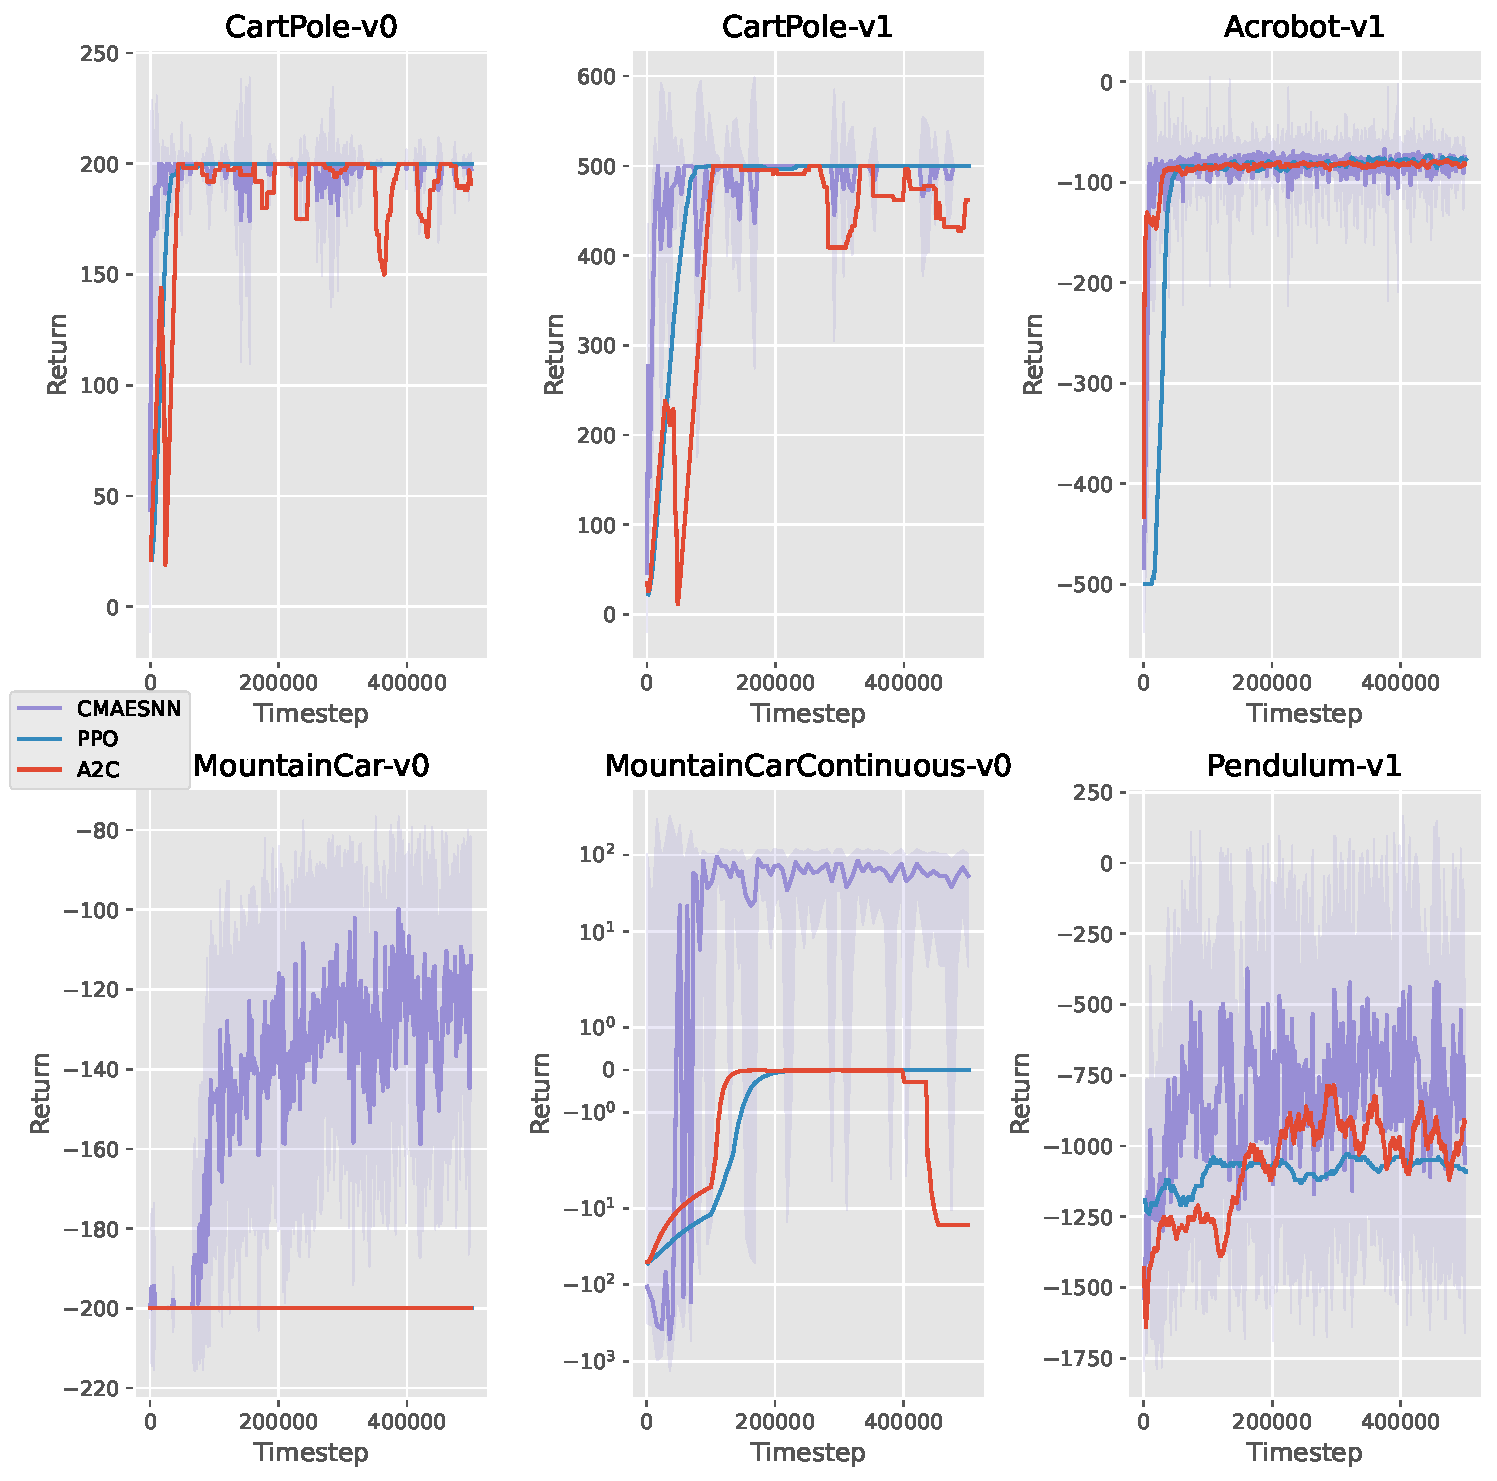
\includegraphics[width=\textwidth]{../plotting/plots/plot_all0.pdf}
    \caption{}
  \end{subfigure}
  \hspace{0.05\textwidth}
  \begin{subfigure}[ht!]{0.35\textwidth}
    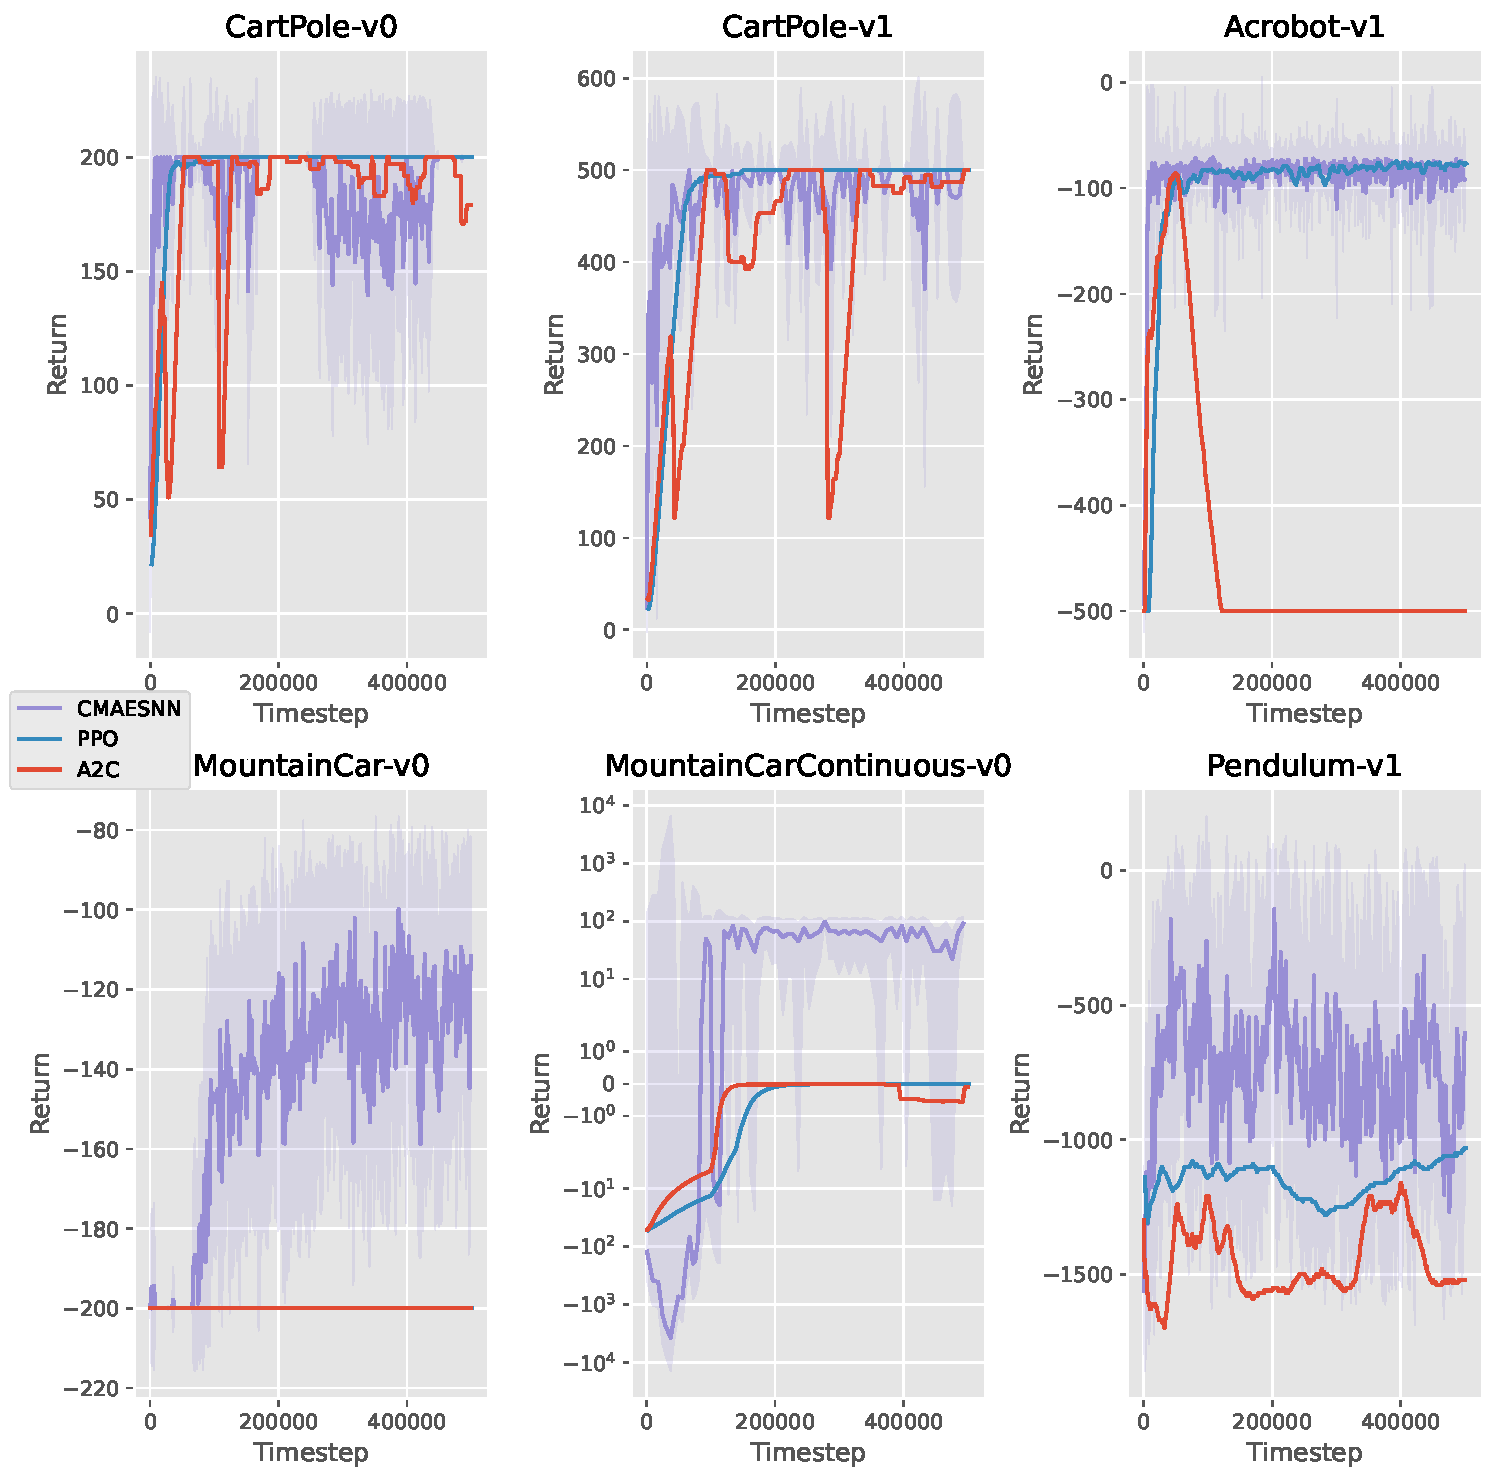
\includegraphics[width=\textwidth]{../plotting/plots/plot_all1.pdf}
    \caption{}
  \end{subfigure}

  \begin{subfigure}[ht!]{0.35\textwidth}
    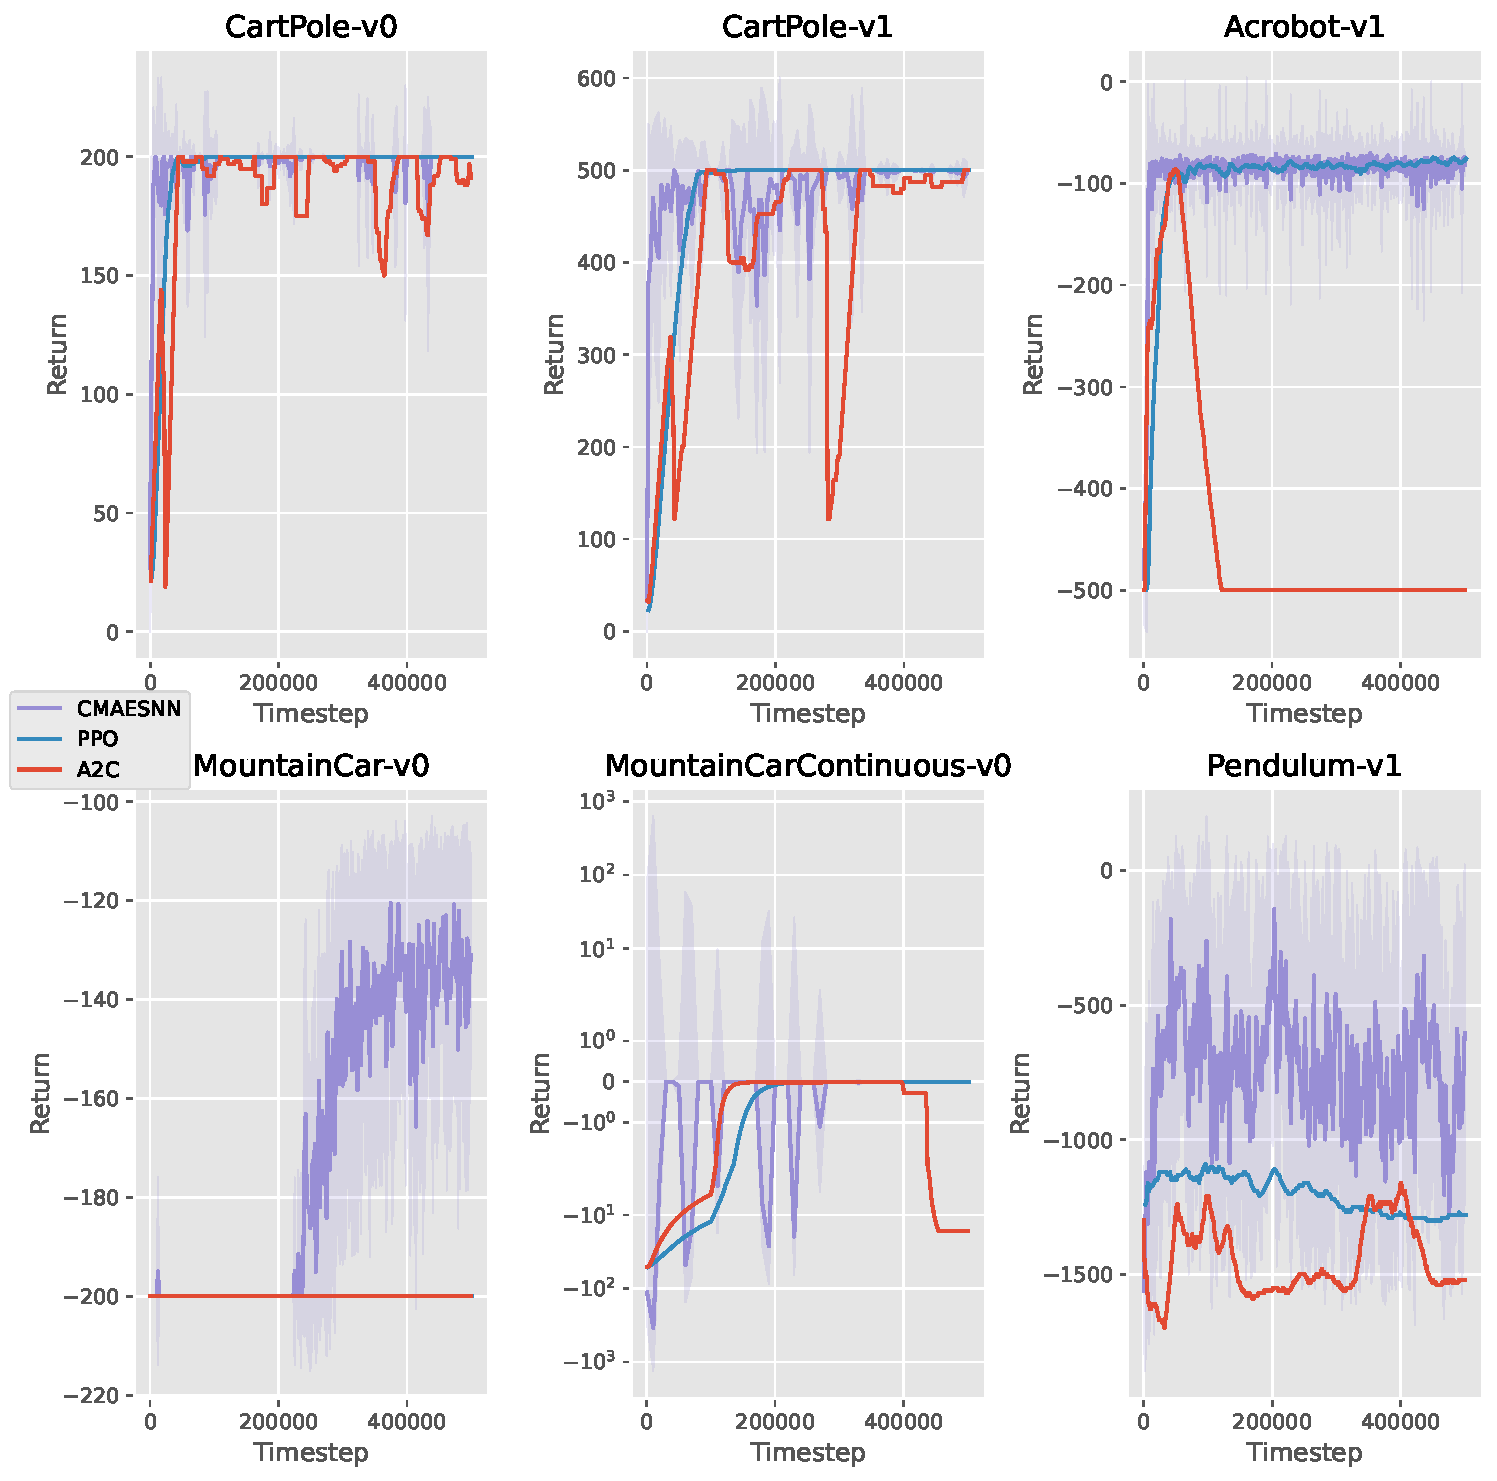
\includegraphics[width=\textwidth]{../plotting/plots/plot_all2.pdf}
    \caption{}
  \end{subfigure}
  \hspace{0.05\textwidth}
  \begin{subfigure}[ht!]{0.35\textwidth}
    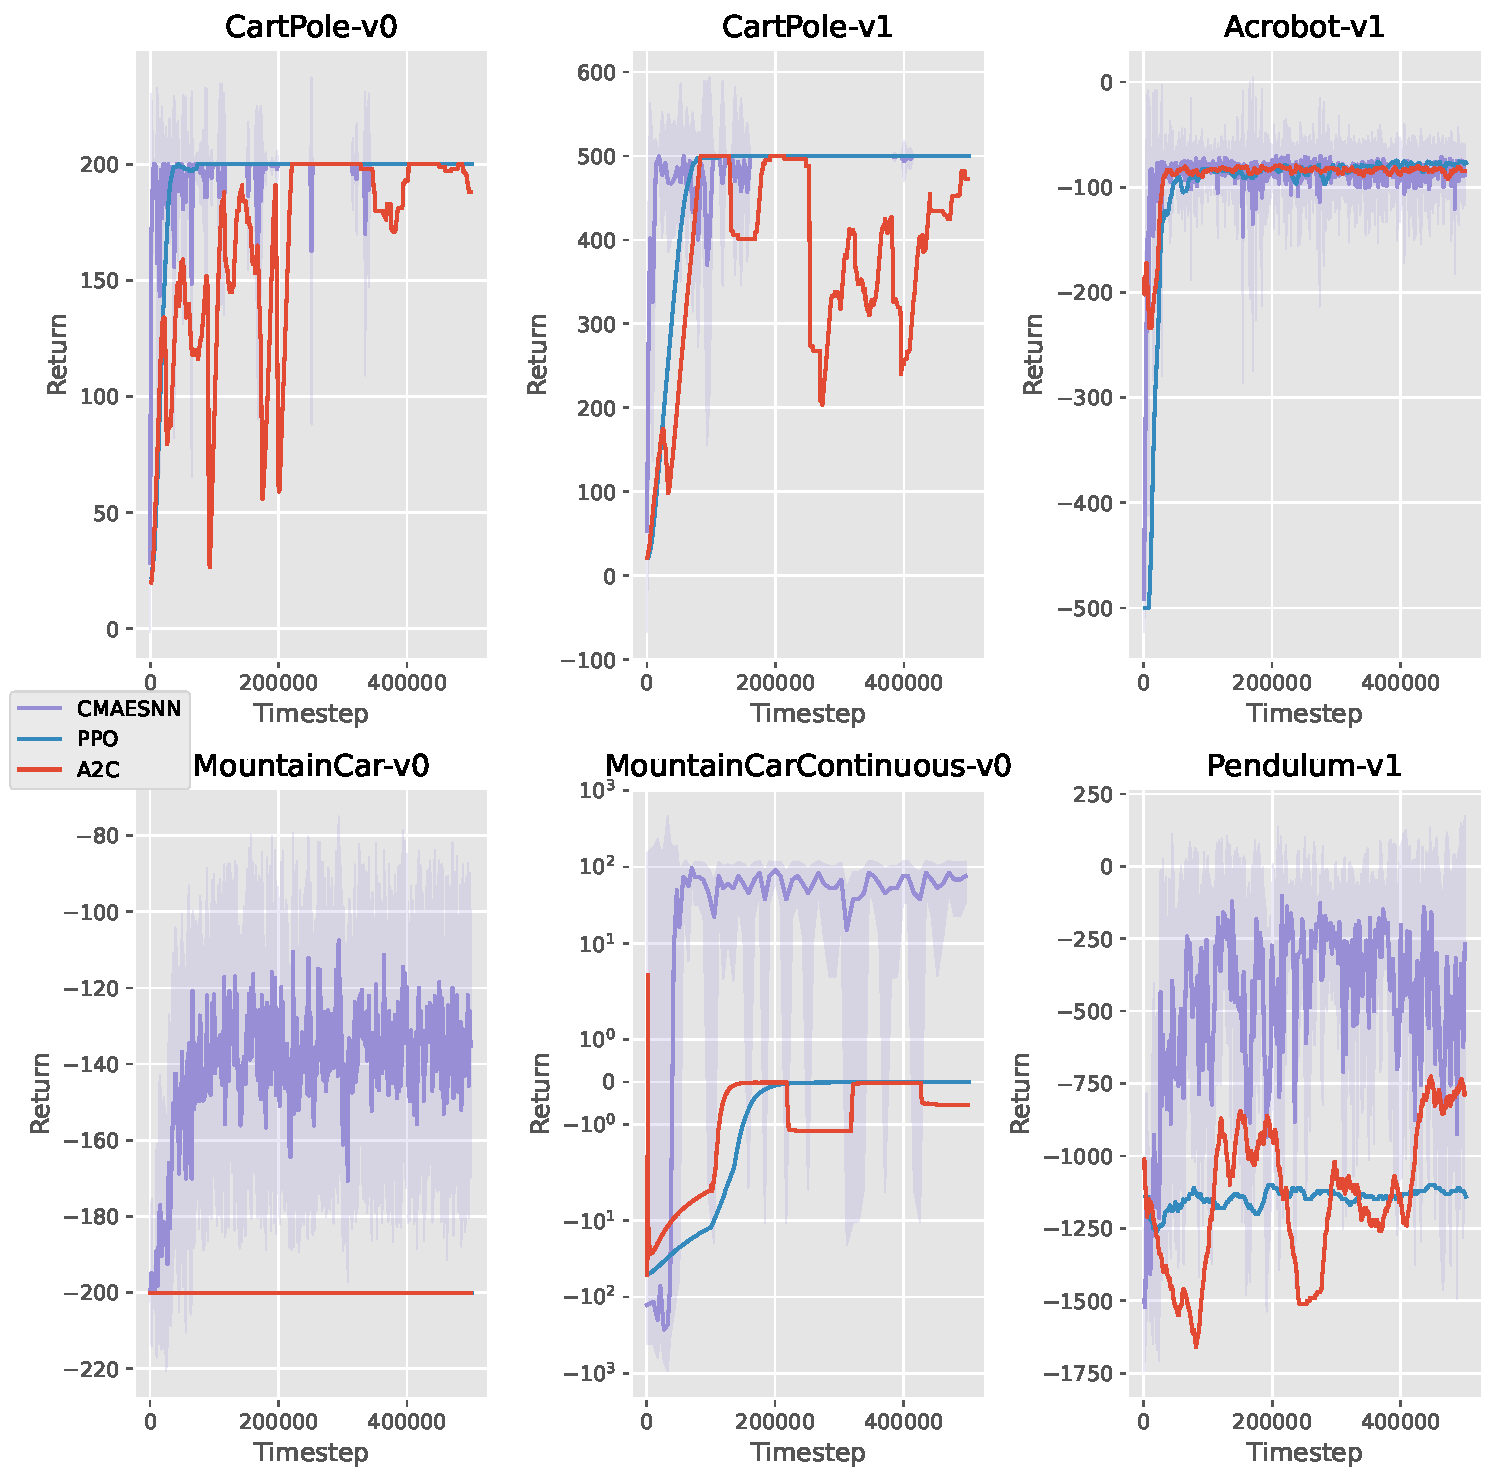
\includegraphics[width=\textwidth]{../plotting/plots/plot_all3.pdf}
    \caption{}
  \end{subfigure}

  \begin{subfigure}[ht!]{0.35\textwidth}
    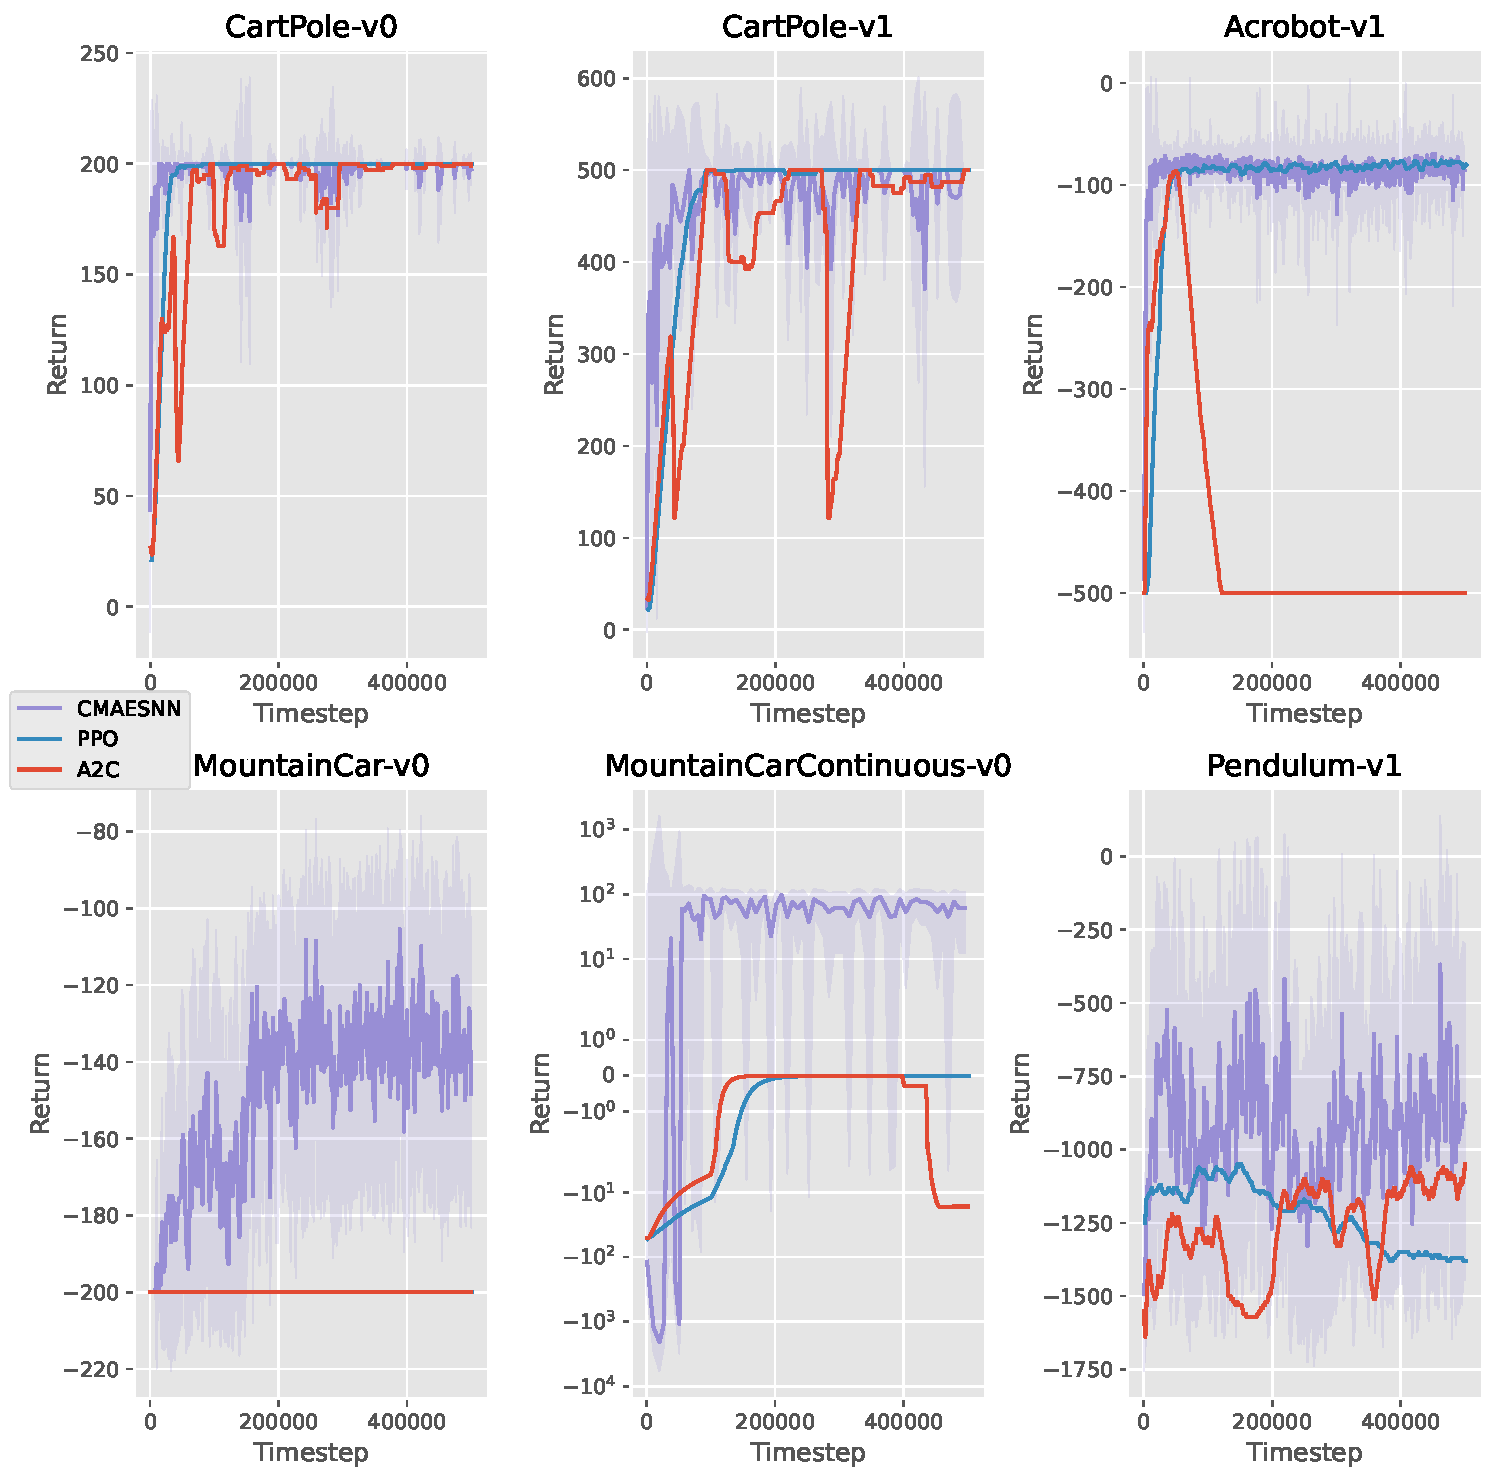
\includegraphics[width=\textwidth]{../plotting/plots/plot_all4.pdf}
    \caption{}
  \end{subfigure}
  \caption{Pięć niezależnych przebiegów uczenia algorytmów w przeciągu 500,000 kroków.
    Algorytmom tym odpowiadają kolory: CMAESNN - fioletowy, PPO - niebieski,
    A2C - czerwony.}
  \label{}

\end{figure}

\pagebreak
\section{Wpływ bias'u na uczenie CMAESNN}\label{appendix:bias}

\begin{figure}[ht!]
  \centering
  \begin{subfigure}[ht!]{0.35\textwidth}
    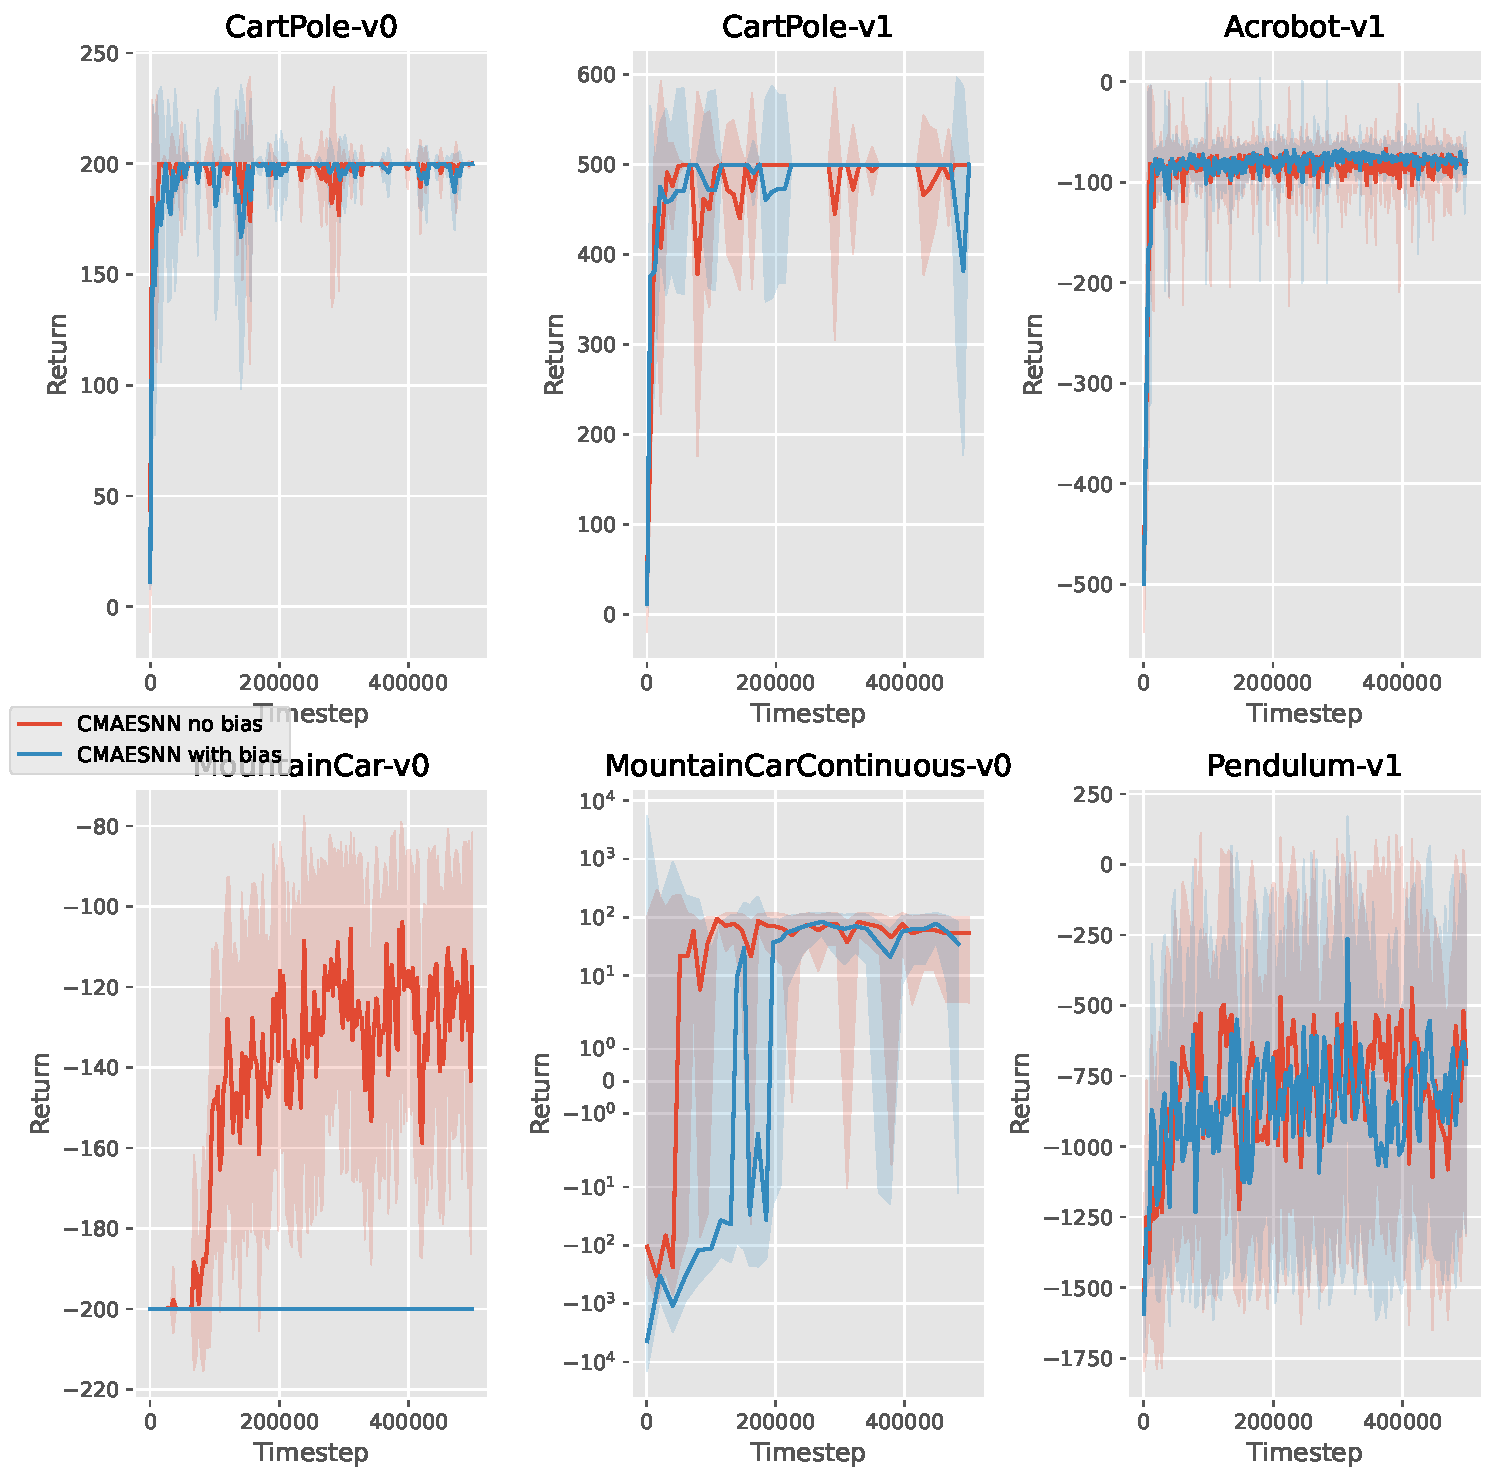
\includegraphics[width=\textwidth]{../plotting/plots/plot_bias_perf0.pdf}
    \caption{}
  \end{subfigure}
  \hspace{0.05\textwidth}
  \begin{subfigure}[ht!]{0.35\textwidth}
    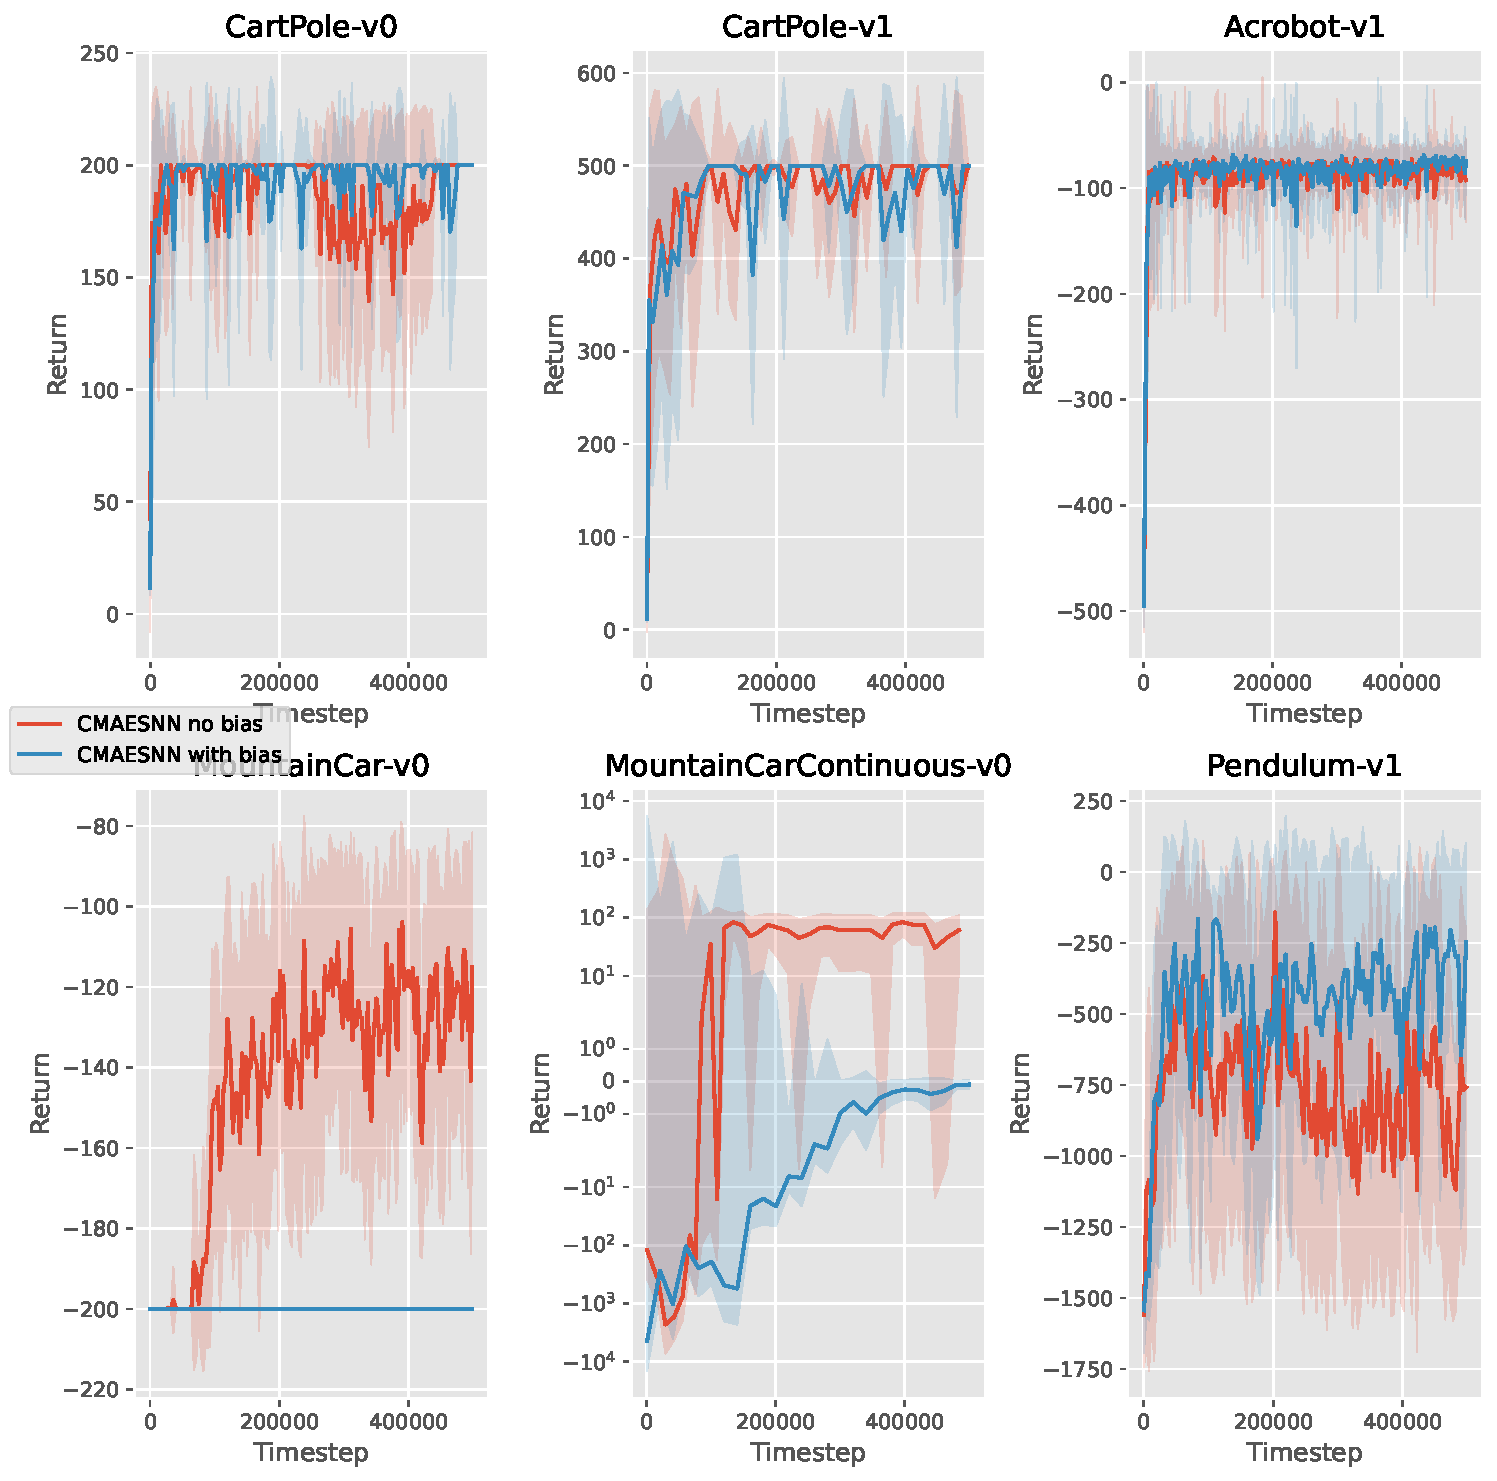
\includegraphics[width=\textwidth]{../plotting/plots/plot_bias_perf1.pdf}
    \caption{}
  \end{subfigure}

  \begin{subfigure}[ht!]{0.35\textwidth}
    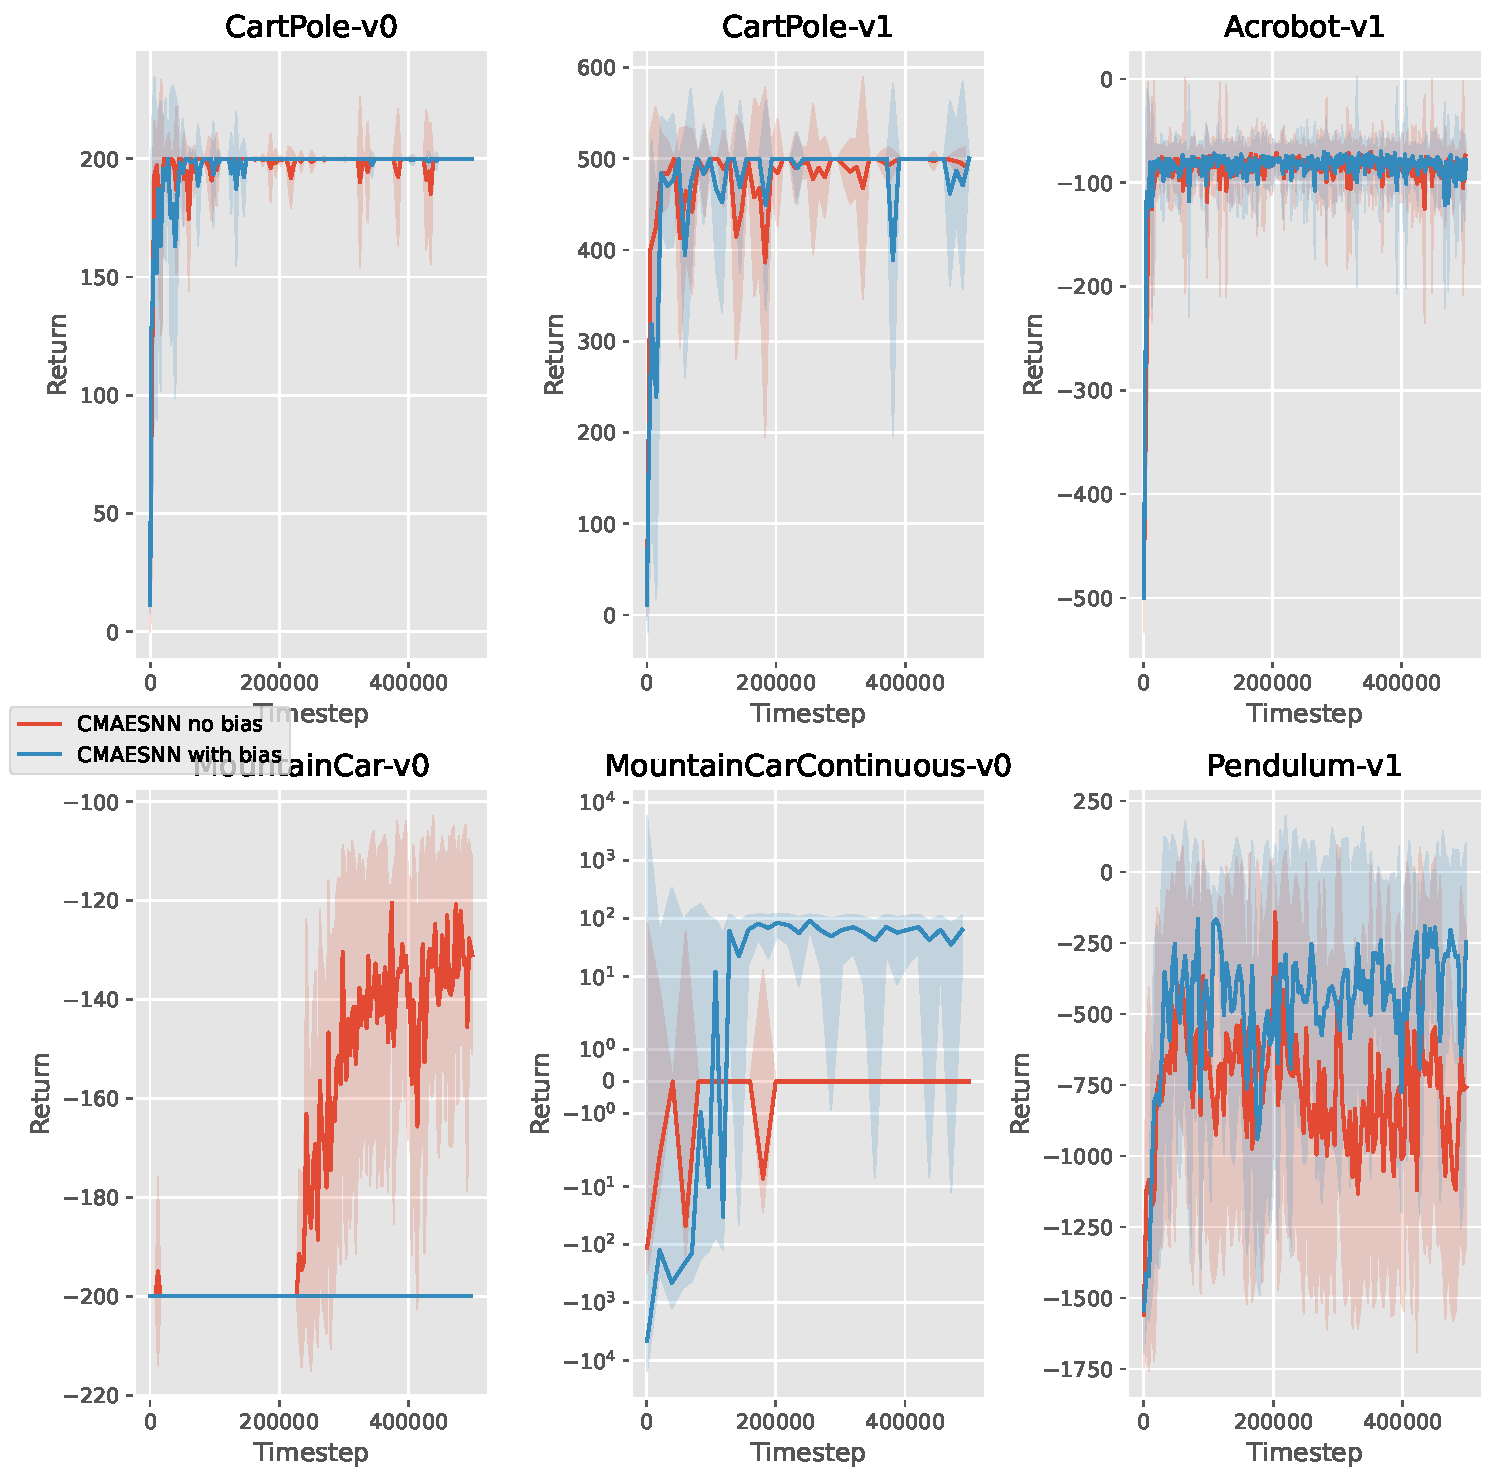
\includegraphics[width=\textwidth]{../plotting/plots/plot_bias_perf2.pdf}
    \caption{}
  \end{subfigure}
  \hspace{0.05\textwidth}
  \begin{subfigure}[ht!]{0.35\textwidth}
    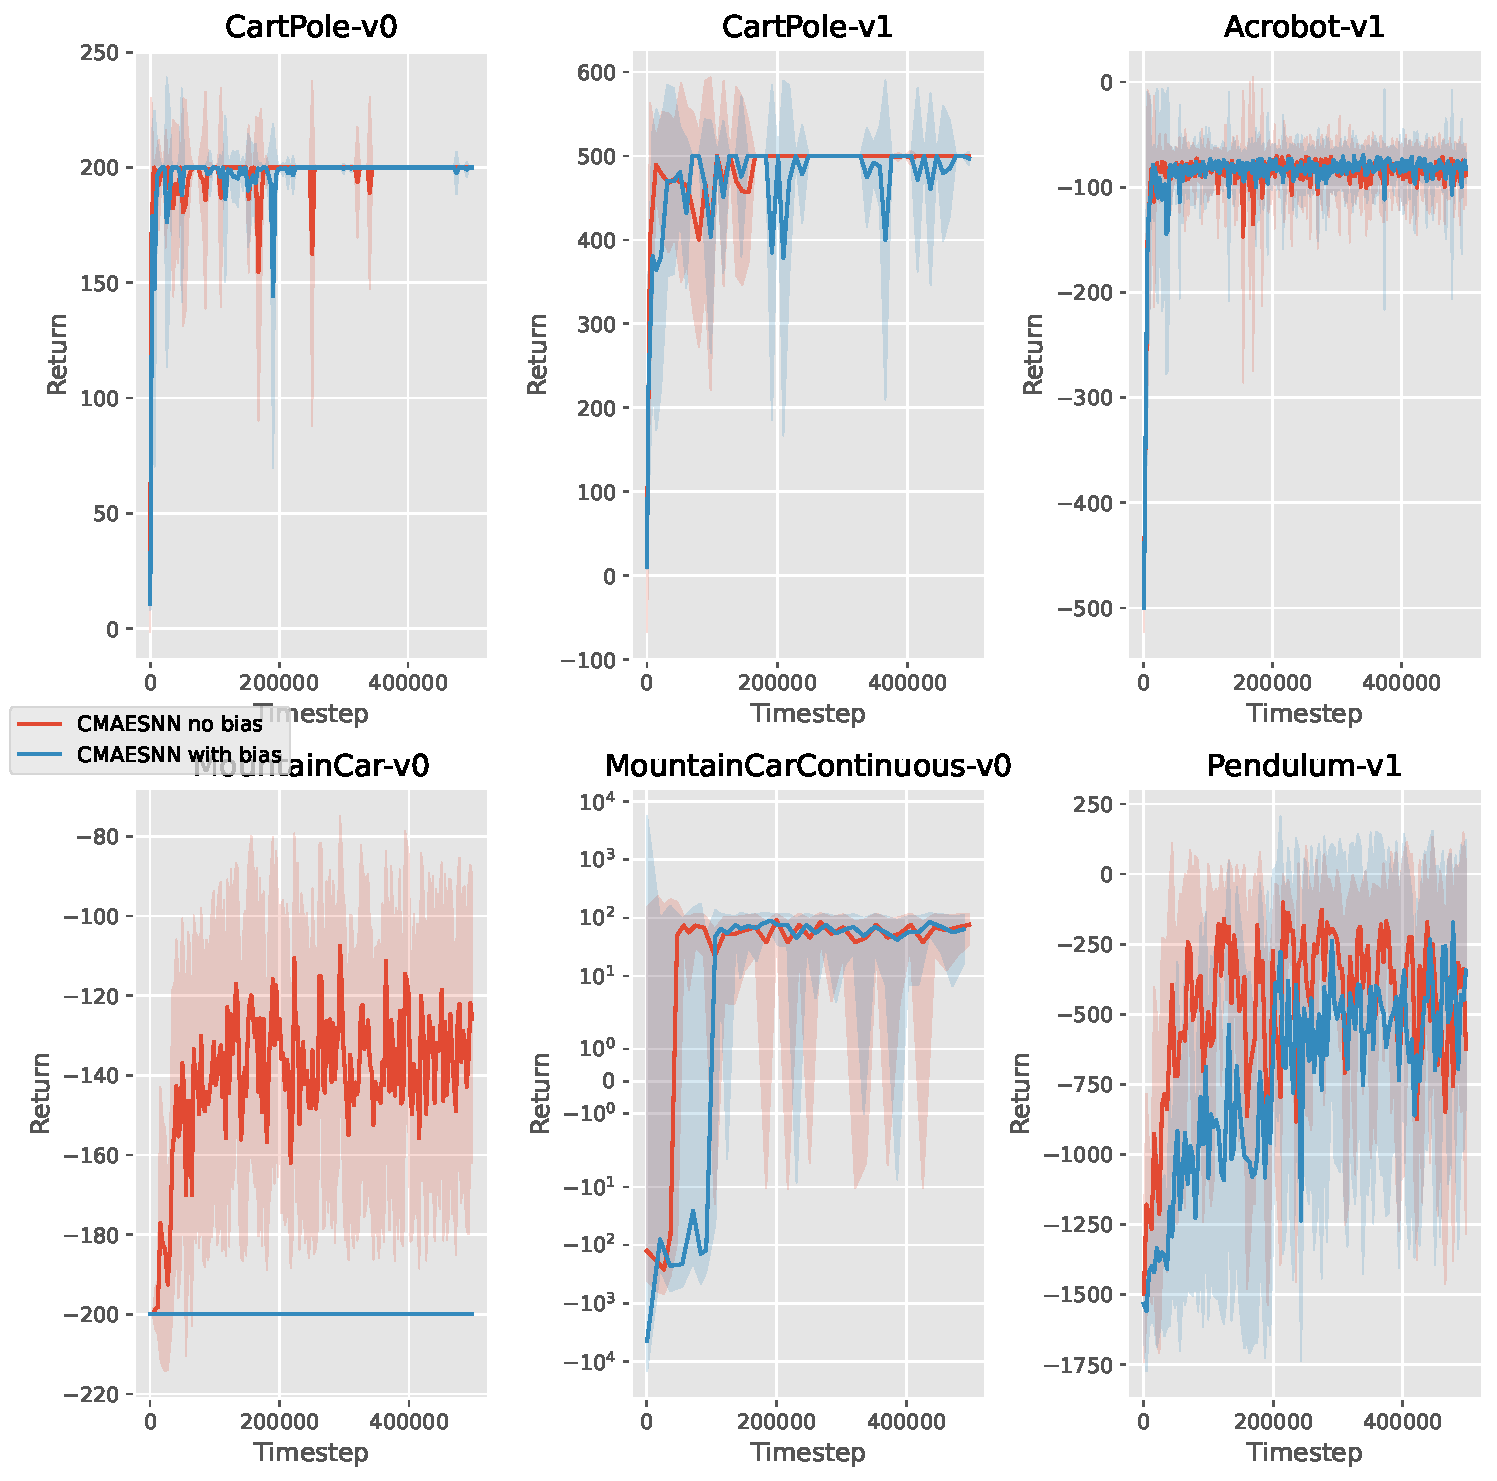
\includegraphics[width=\textwidth]{../plotting/plots/plot_bias_perf3.pdf}
    \caption{}
  \end{subfigure}

  \begin{subfigure}[ht!]{0.35\textwidth}
    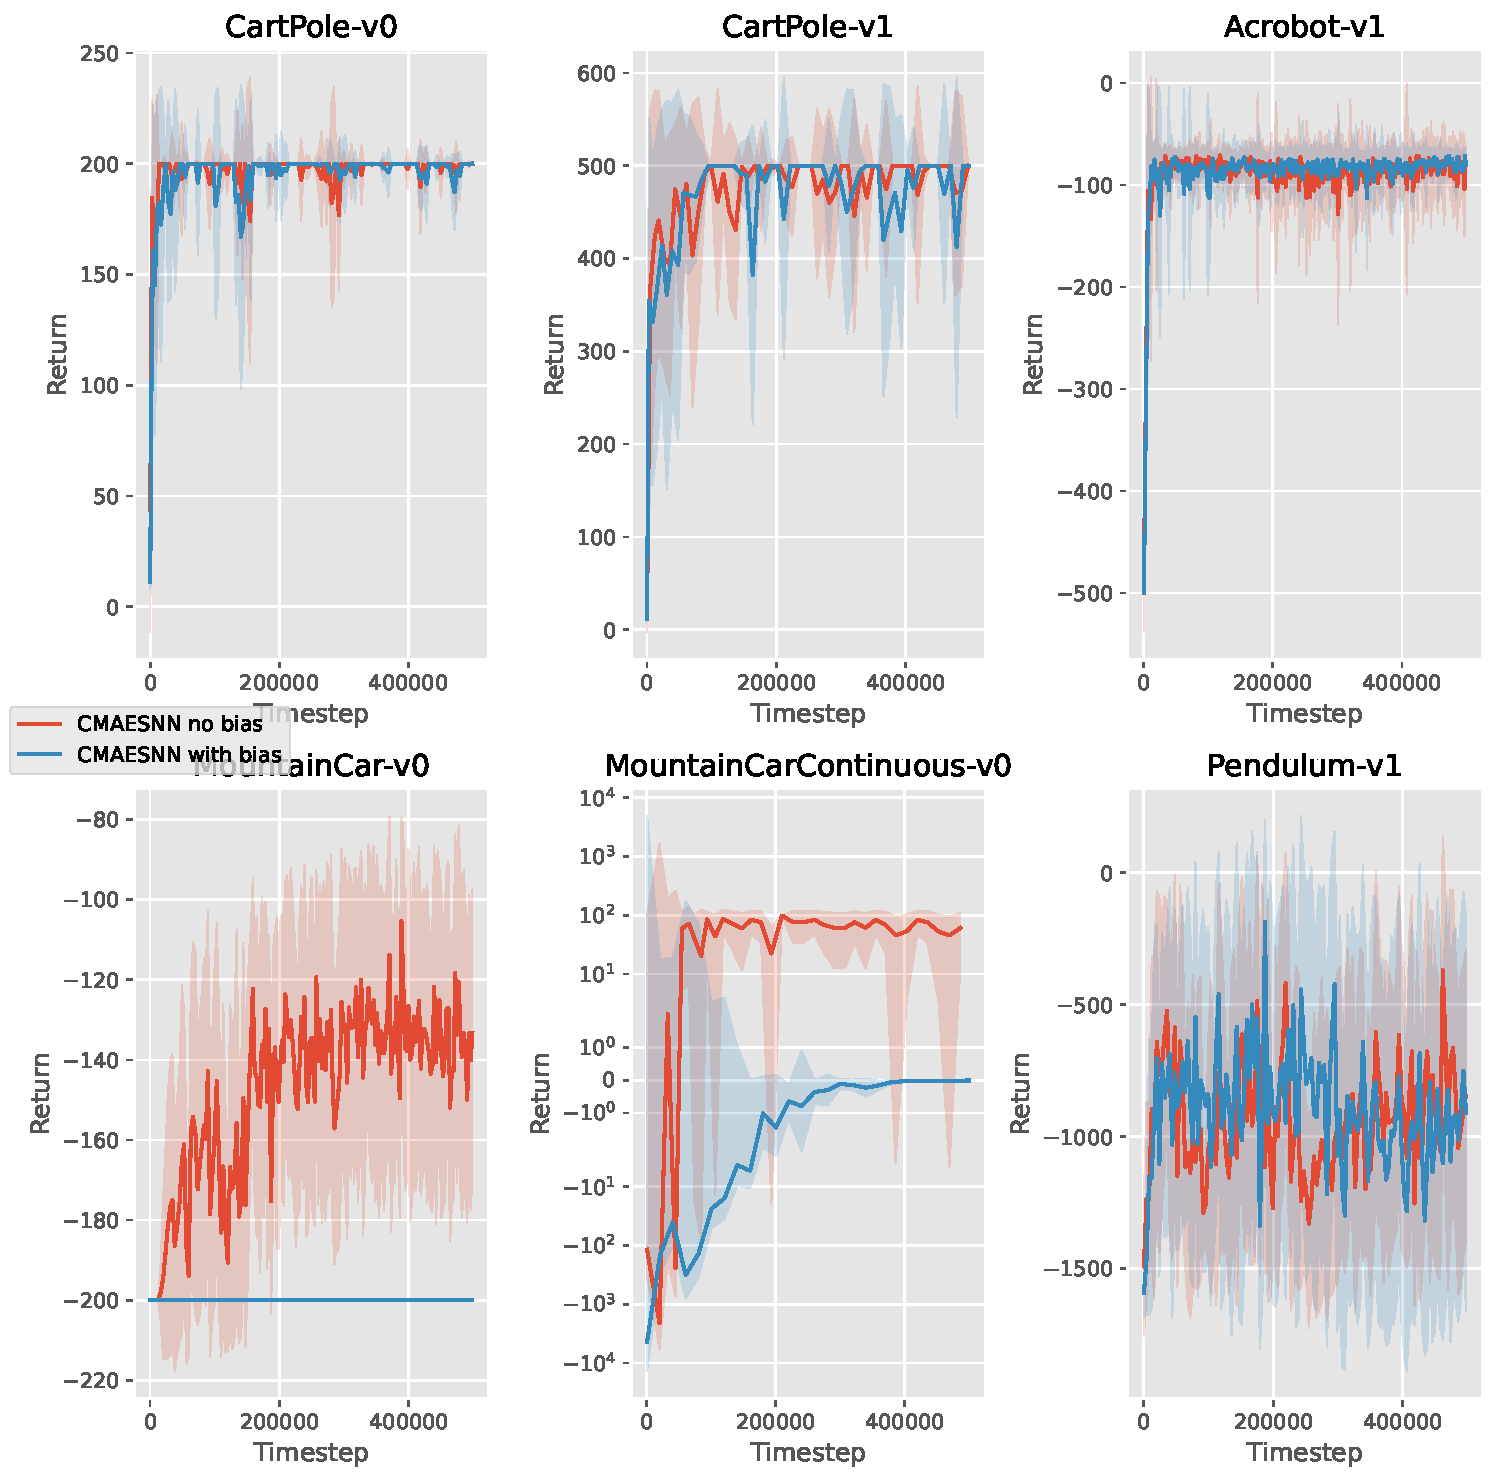
\includegraphics[width=\textwidth]{../plotting/plots/plot_bias_perf4.pdf}
    \caption{}
  \end{subfigure}
  \caption{Pięć niezależnych przebiegów uczenia algorytmów CMAESNN
    z (niebieski) i bez (czerwony) dodatkowymi parametrami bias.
    Uczenie dokonywało się w przeciągu 500,000 kroków.}
\end{figure}

\end{document}
